\documentclass[11pt, oneside]{article}
\usepackage[letterpaper, margin=2cm]{geometry}
\usepackage{MATH667}

\begin{document}
\noindent \textbf{\Large{Caleb Logemann \\
MATH667 Hyperbolic Partial Differential Equations \\
Homework 1
}}

%\lstinputlisting[language=MATLAB]{H01_23.m}
\begin{enumerate}
  \item % #1 Done
    For constant coefficient linear wave equation initial value problem
    \[
      \begin{cases}
        u_t + a u_x = 0 \\
        u(x, 0) = u_0(x)
      \end{cases}
    \]
    for all $x \in \RR$ and $t \ge 0$, verify that the solution
    $u(x, t) = u_0(x - at)$ satisfies the following integral form.
    We assume the initial $u_0(x)$ is a smooth function.
    \[
      \dintt{x_1}{x_2}{u(x, t_2)}{x} = \dintt{x_1}{x_2}{u(x, t_1)}{x} +
      \dintt{t_1}{t_2}{au(x_1, t)}{t} - \dintt{t_1}{t_2}{au(x_2, t)}{t}, \quad
      \forall x_1, x_2 \in \RR, \forall t_1, t_2 \ge 0.
    \]

    Let $U$ be an antiderivative of $u_0$, that is
    $\dintt{y_1}{y_2}{u_0(y)}{y} = U(y_2) - U(y_1)$.
    This is guaranteed to exist since $u_0$ is a smooth function.
    Now we can consider each of the terms of the integral form seperately.
    The first term can be simplified as follows,
    \begin{align*}
      \dintt{x_1}{x_2}{u(x, t_2)}{x} &= \dintt{x_1}{x_2}{u_0(x - at_2)}{x} \\
      &= U(x_2 - at_2) - U(x_1 - at_2).
    \end{align*}
    The second term is
    \begin{align*}
      \dintt{x_1}{x_2}{u(x, t_1)}{x} &= \dintt{x_1}{x_2}{u_0(x - at_1)}{x} \\
      &= U(x_2 - at_1) - U(x_1 - at_1).
    \end{align*}
    The third term is
    \begin{align*}
      \dintt{t_1}{t_2}{au(x_1, t)}{t} &= \dintt{t_1}{t_2}{au_0(x_1 - at)}{t} \\
      &= \frac{a}{-a} \p{U(x_1 - at_2) - U(x_1 - at_1)} \\
      &= - U(x_1 - at_2) + U(x_1 - at_1).
    \end{align*}
    The last term becomes
    \begin{align*}
      \dintt{t_1}{t_2}{au(x_2, t)}{t} &= \dintt{t_1}{t_2}{au_0(x_2 - at)}{t} \\
      &= \frac{a}{-a} \p{U(x_1 - at_2) - U(x_1 - at_1)} \\
      &= -U(x_2 - at_2) + U(x_2 - at_1).
    \end{align*}

    Combining these four terms back into the integral form gives.
    \begin{align*}
      U(x_2 - at_2) - U(x_1 - at_2) &= U(x_2 - at_1) - U(x_1 - at_1) - U(x_1 - at_2) \\
        &+ U(x_1 - at_1) + U(x_2 - at_2) - U(x_2 - at_1) \\
      U(x_2 - at_2) - U(x_1 - at_2) &= - U(x_1 - at_2) + U(x_2 - at_2) \\
      - U(x_1 - at_2) &= - U(x_1 - at_2)  \\
      0 &= 0
    \end{align*}
    This shows that the integral form is satisfied for all values of $x_1, x_2 \in \RR$ and $t_1, t_2 \ge 0$.

  \item % #2 Done
    For viscous Burger's equation $u_t + uu_x + \varepsilon u_{xx}$ with initial condition
    \[
      u(x, 0) =
      \begin{cases}
        1 & x \le 0 \\
        0 & x > 0
      \end{cases},
    \]
    verify the traveling wave solution $u_{\varepsilon}(x, t)$ satisfies the given PDE.\@
    We have $u_{\varepsilon}(x, t) = w(x - \frac{1}{2}t)$, where
    $w(y) = \frac{1}{2}\p{1 - \tanh{\frac{y}{4\varepsilon}}}$.
    Graph the solution $u_{\varepsilon}(x, t)$ at $t = 1$ with
    $\varepsilon = 10^{-2}, 10^{-4}, 10^{-6}$.

    First note that
    \begin{align*}
      u_{\varepsilon, t} &= -\frac{1}{2} w'\p{x - \frac{1}{2}t} \\
      u_{\varepsilon, x} &= w'\p{x - \frac{1}{2}t} \\
      u_{\varepsilon, xx} &= w''\p{x - \frac{1}{2}t}.
    \end{align*}
    Also note the derivatives of $w$ are
    \begin{align*}
      w'(y) = -\frac{1}{8\varepsilon} \p{1 - \tanh[2]{\frac{y}{4\varepsilon}}} \\
      w''(y) = \frac{1}{16\varepsilon^2} \tanh{\frac{y}{4\varepsilon}} \p{1 - \tanh[2]{\frac{y}{4\varepsilon}}} \\
    \end{align*}
    Now we see that
    \begin{align*}
      u_{\varepsilon, t} &= \frac{1}{16\varepsilon} \p{1 - \tanh[2]{\frac{x - \frac{1}{2}t}{4\varepsilon}}}\\
      u_{\varepsilon, x} &= -\frac{1}{8\varepsilon} \p{1 - \tanh[2]{\frac{x - \frac{1}{2}t}{4\varepsilon}}} \\
      u_{\varepsilon, xx} &= \frac{1}{16\varepsilon^2} \tanh{\frac{x - \frac{1}{2}t}{4\varepsilon}} \p{1 - \tanh[2]{\frac{x - \frac{1}{2}t}{4\varepsilon}}}.
    \end{align*}
    Plugging these into the left hand side and right hand side of the PDE gives the following.
    First I will simplify the left hand side
    \begin{gather*}
      u_{\varepsilon, t} + u_{\varepsilon} u_{\varepsilon, x} \\
      \frac{1}{16\varepsilon} \p{1 - \tanh[2]{\frac{x - \frac{1}{2}t}{4\varepsilon}}} + -\frac{1}{2}\p{1 - \tanh{\frac{x - \frac{1}{2}t}{4\varepsilon}}}\frac{1}{8\varepsilon} \p{1 - \tanh[2]{\frac{x - \frac{1}{2}t}{4\varepsilon}}} \\
      \frac{1}{16\varepsilon} - \frac{1}{16\varepsilon}\tanh[2]{\frac{x - \frac{1}{2}t}{4\varepsilon}} + \p{-\frac{1}{16\varepsilon} + \frac{1}{16\varepsilon}\tanh{\frac{x - \frac{1}{2}t}{4\varepsilon}}} \p{1 - \tanh[2]{\frac{x - \frac{1}{2}t}{4\varepsilon}}} \\
      \frac{1}{16\varepsilon} - \frac{1}{16\varepsilon}\tanh[2]{\frac{x - \frac{1}{2}t}{4\varepsilon}} + -\frac{1}{16\varepsilon} + \frac{1}{16\varepsilon}\tanh{\frac{x - \frac{1}{2}t}{4\varepsilon}} + \frac{1}{16\varepsilon}\tanh[2]{\frac{x - \frac{1}{2}t}{4\varepsilon}} - \frac{1}{16\varepsilon}\tanh[3]{\frac{x - \frac{1}{2}t}{4\varepsilon}} \\
      \frac{1}{16\varepsilon}\tanh{\frac{x - \frac{1}{2}t}{4\varepsilon}} - \frac{1}{16\varepsilon}\tanh[3]{\frac{x - \frac{1}{2}t}{4\varepsilon}}.
    \end{gather*}
    Next I will simplify the right hand side
    \begin{gather}
      \varepsilon u_{\varepsilon, xx} \\
      \varepsilon \frac{1}{16\varepsilon^2} \tanh{\frac{x - \frac{1}{2}t}{4\varepsilon}} \p{1 - \tanh[2]{\frac{x - \frac{1}{2}t}{4\varepsilon}}} \\
      \frac{1}{16\varepsilon} \p{\tanh{\frac{x - \frac{1}{2}t}{4\varepsilon}} - \tanh[3]{\frac{x - \frac{1}{2}t}{4\varepsilon}}} \\
    \end{gather}
    We see that this is equal to the left hand side shown previously, so $u_{\varepsilon}(x, t)$ does satisfy the PDE.\@

    Also $u_{\varepsilon}(x, t)$ satisfies the inital conditions as $\varepsilon \to 0$.
    To see this consider the following
    \begin{align*}
      \lim[\varepsilon \to 0]{u_{\varepsilon}(x, 0)} &= \lim[\varepsilon \to 0]{\frac{1}{2}\p{1 - \tanh{\frac{x}{3\varepsilon}}}} \\
      &= \frac{1}{2} - \lim[\varepsilon \to 0]{\tanh{\frac{x}{4\varepsilon}}}
      \intertext{If $x \le 0$, then this is equivalent to}
      &= \frac{1}{2} - \lim[y \to -\infty]{\tanh{y}} \\
      &= \frac{1}{2} - -\frac{1}{2} = 1
      \intertext{If $x > 0$, then this limit is equivalent to}
      &= \frac{1}{2} - \lim[y \to \infty]{\tanh{y}} \\
      &= \frac{1}{2} - \frac{1}{2} = 0
    \end{align*}
    This shows that $u_{\varepsilon}(x, t)$ satisfies the initial conditions as $\varepsilon \to 0$.

    The following is a graph of $u_{\varepsilon}(x, 1)$ with $\varepsilon = 10^{-2}, 10^{-4}, 10^{-6}$.
    Note that graph for $\varepsilon = 10^{-4}$ and the graph for
    $\varepsilon = 10^{-6}$ are almost directly on top of on another.
    \begin{center}
      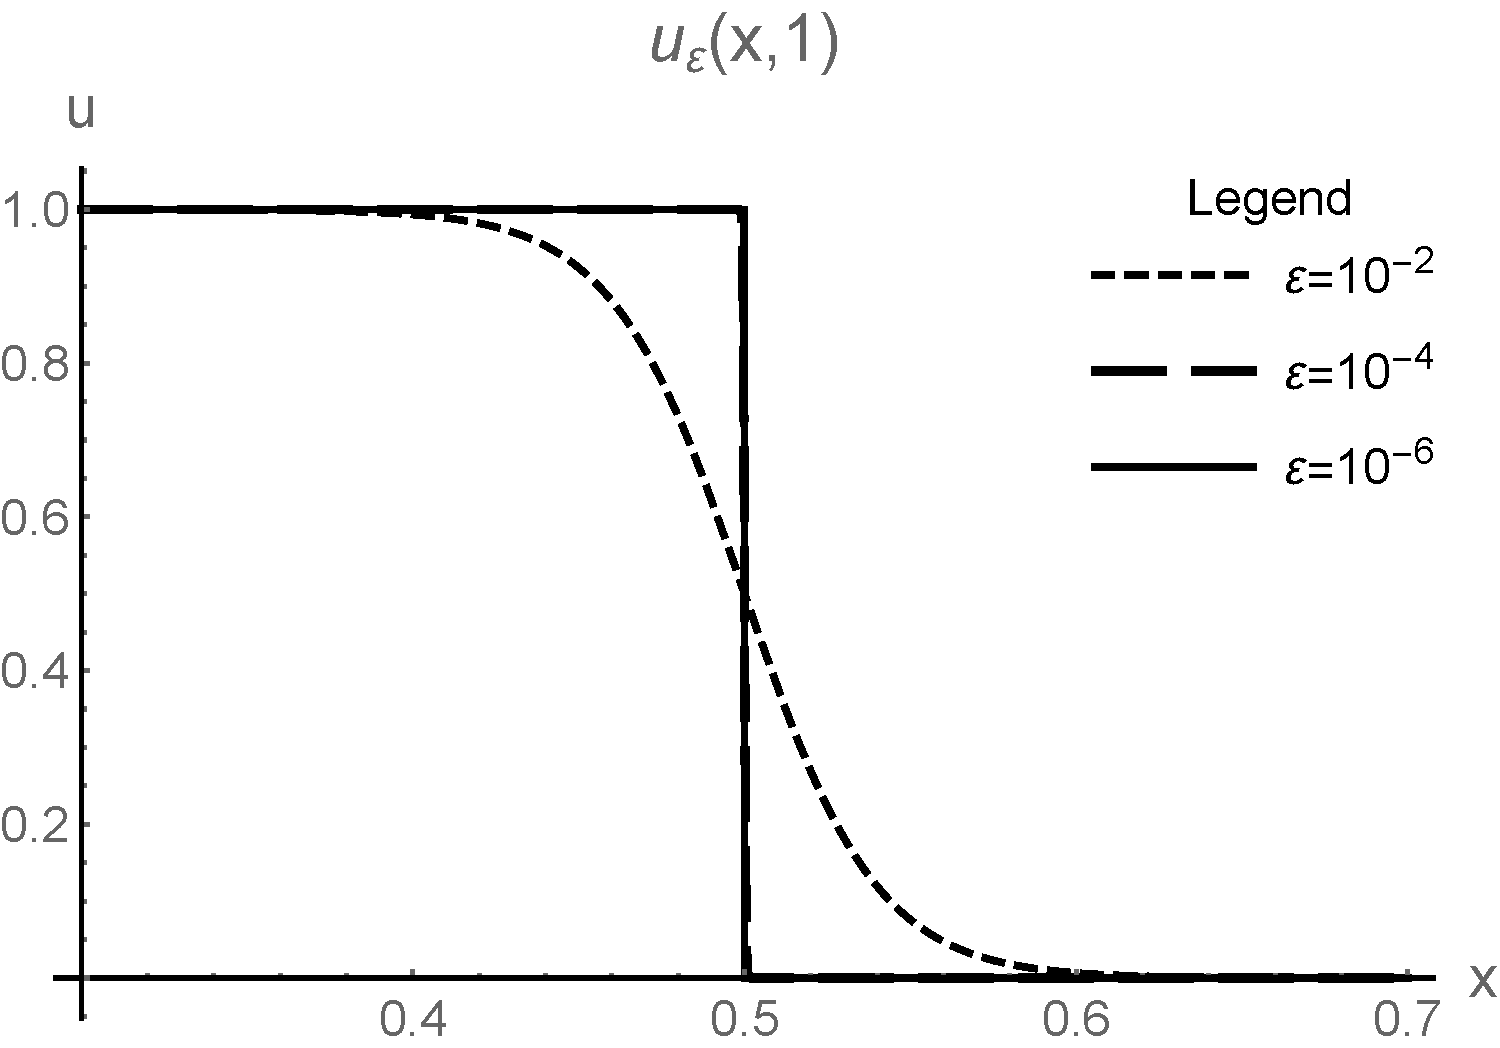
\includegraphics[scale=.5]{Figures/01_01}
    \end{center}

  \item % #3
    For Burger's equation Riemann problem
    \[
      u(x, 0) =
      \begin{cases}
        u_l & x \le 0 \\
        u_r & x > 0
      \end{cases}
    \]
    with $u_l < u_r$, show that
    \[
      u(x, t) =
      \begin{cases}
        u_l & x < s_m t \\
        u_m & s_m t \le x \le u_m t \\
        \frac{x}{t} & u_m t \le x \le u_r t \\
        u_r & u_r t \le x
      \end{cases}
    \]
    is a weak solution.
    Let $u_l < u_m < u_r$ and $s_m = (u_l + u_r)/2$.
    Sketch the characteristics for this solution.

    Weak solutions of Burger's equation satisfy the following
    \[
      \dintt{0}{\infty}{\dintt{-\infty}{\infty}{u \phi_t + \frac{1}{2} u^2 \phi_x}{x}}{t} = -\dintt{-\infty}{\infty}{u(x, 0)\phi(x, 0)}{x}
    \]
    for all test functions $\phi \in C^{1}_0(\RR^2 \times \RR^+)$.
    I will consider the integral equation in three parts.
    First consider
    \[
      \dintt{0}{\infty}{\dintt{-\infty}{\infty}{u \phi_t}{x}}{t}
    \]
    This can be simplified by splitting the integral in space and time,
    substituting in for $u$ and then integrating by parts.
    This integral can be broken down in several different ways depending on the
    values of $u_l$, $u_m$, and $u_r$.
    There are in fact four different cases, shown below.
    \begin{center}
      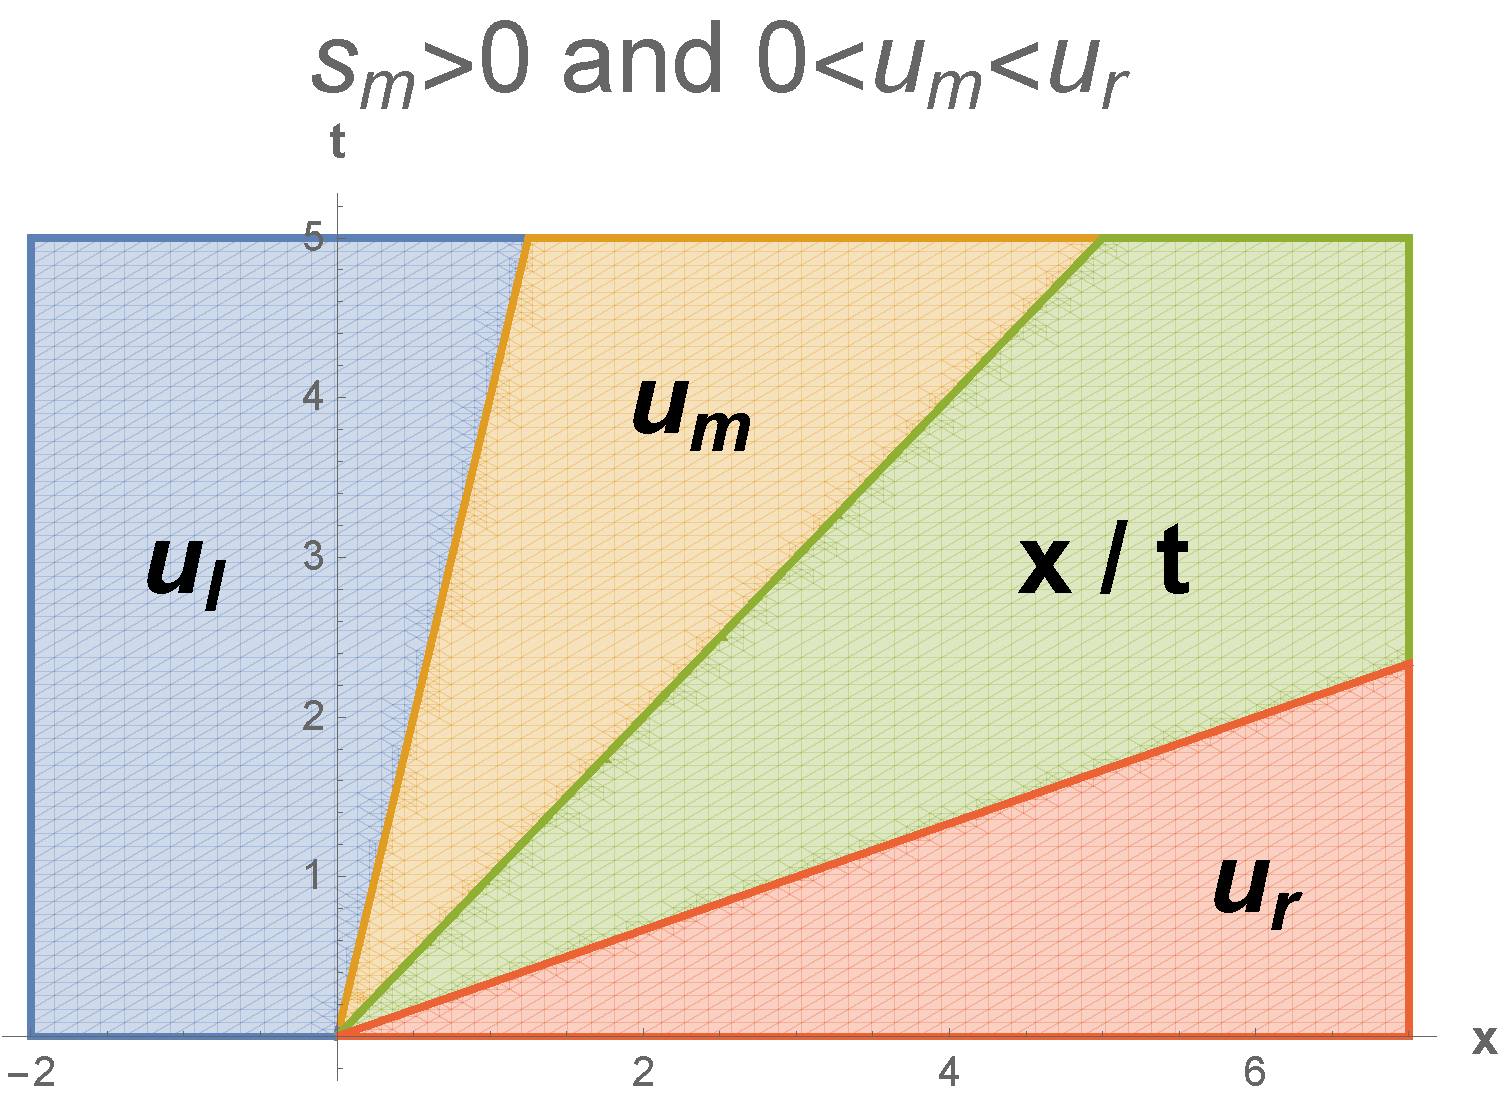
\includegraphics[scale=.30]{Figures/01_03.pdf}
      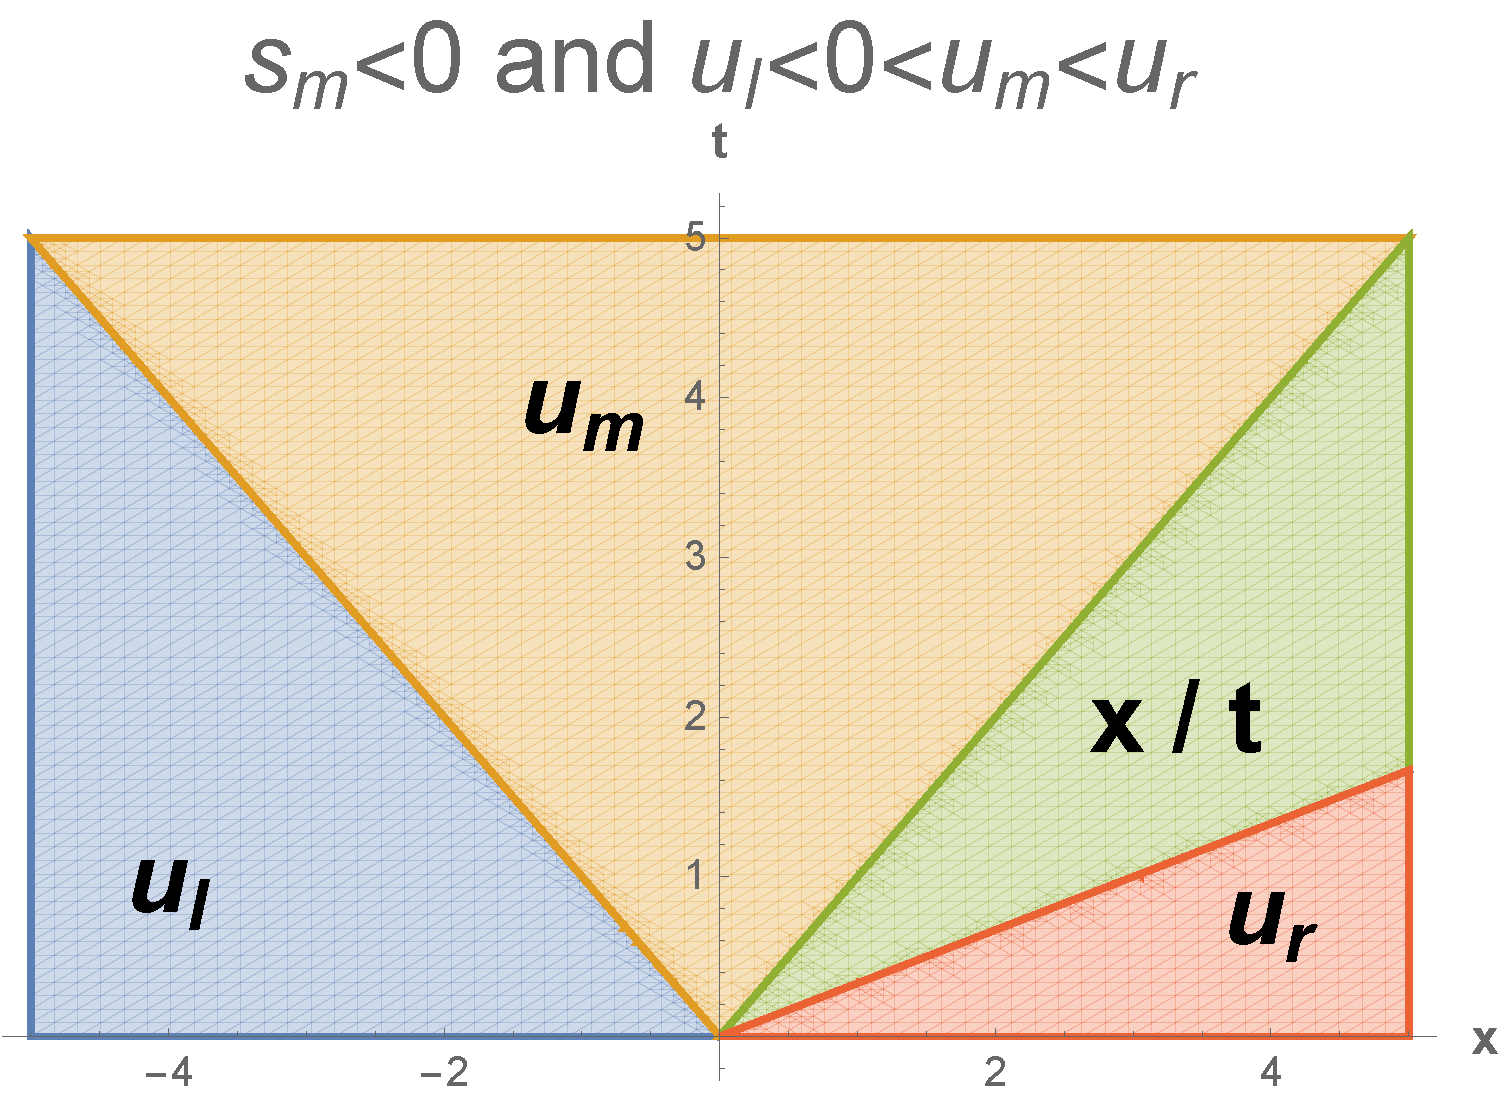
\includegraphics[scale=.30]{Figures/01_04.pdf}
      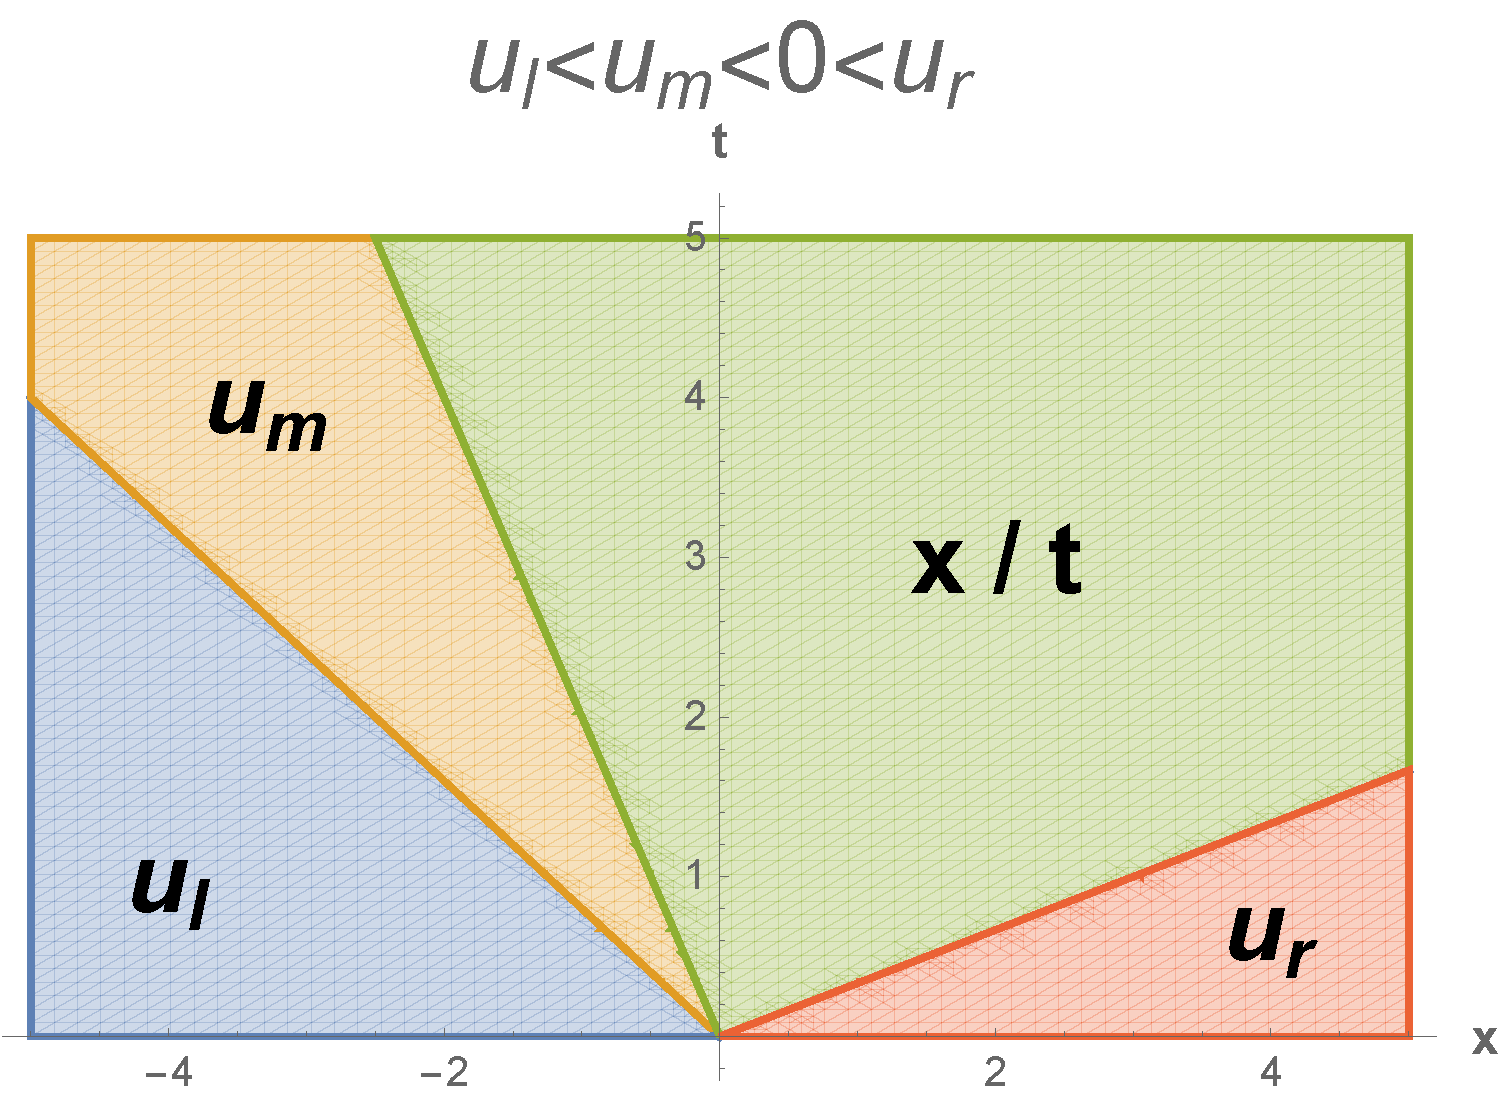
\includegraphics[scale=.30]{Figures/01_05.pdf}
      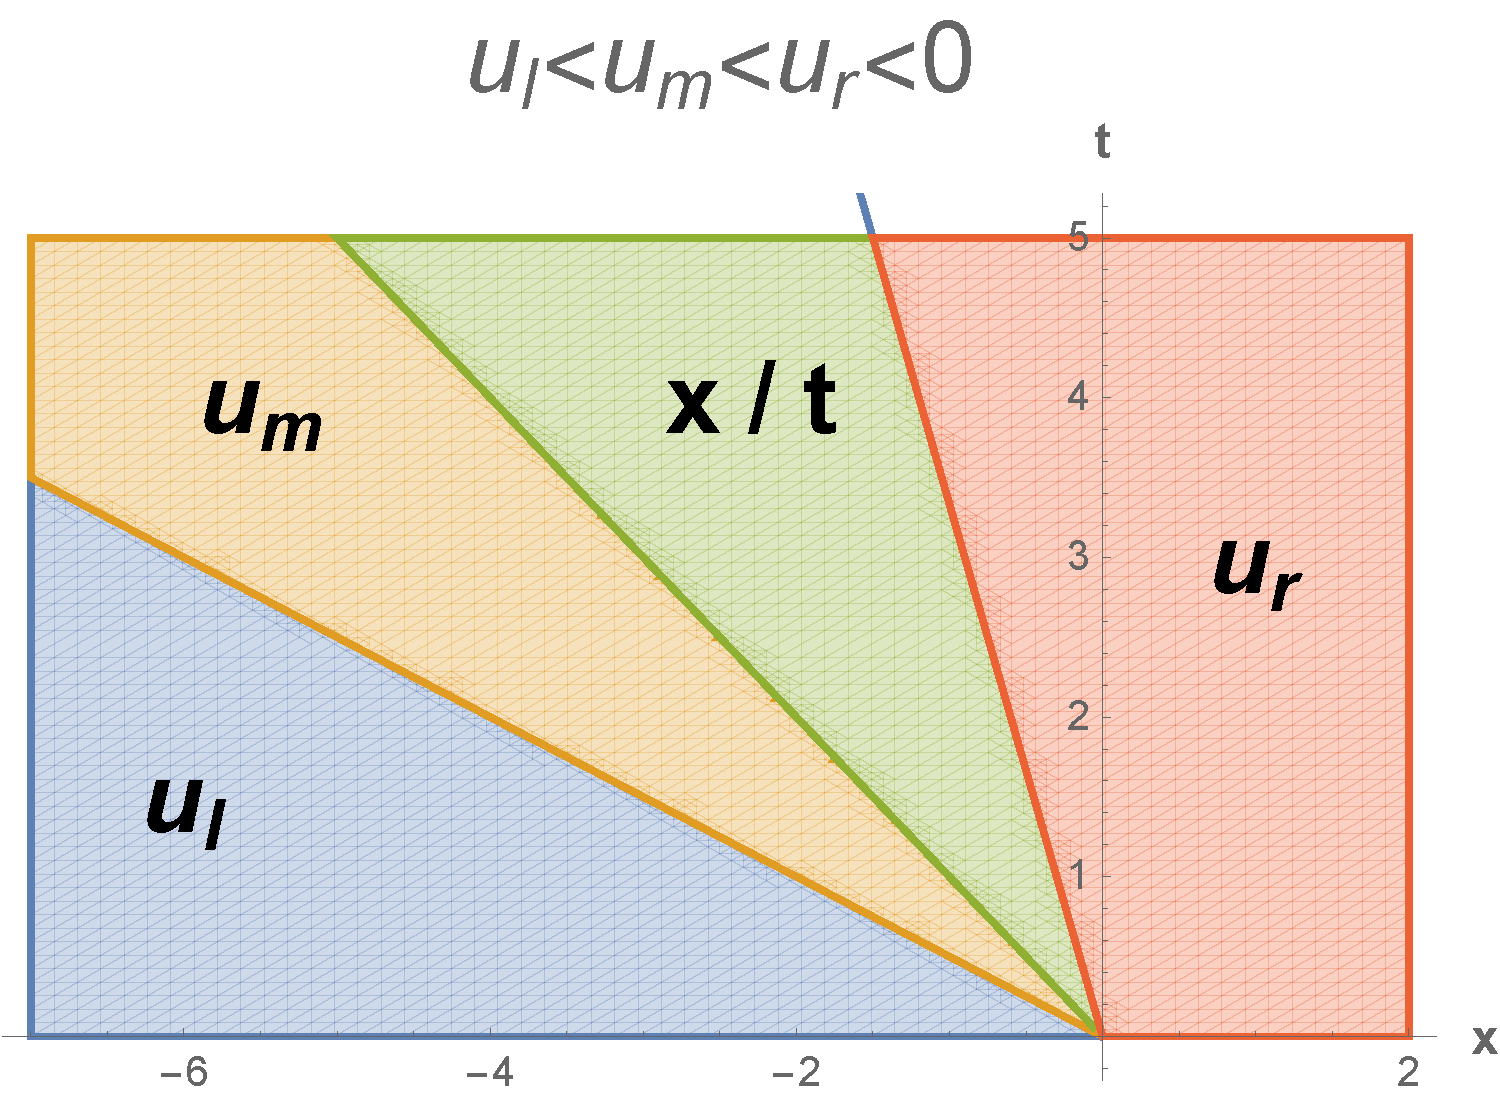
\includegraphics[scale=.30]{Figures/01_06.pdf}
    \end{center}
    I will only consider the case where $s_m > 0$, this implies that $0 < u_m < u_r$.
    $u_l$ may be positive or negative but it is large enough that $s_m > 0$.
    The other cases are roughly equivalent and would be redundant to fully write up.
    In this case we can revisit the previous integral split it up into left and
    right quadrants as follows.
    \begin{align*}
      \dintt{0}{\infty}{\dintt{-\infty}{\infty}{u \phi_t}{x}}{t} 
      &= \dintt{-\infty}{\infty}{\dintt{0}{\infty}{u \phi_t}{t}}{x} \\
      &= \dintt{-\infty}{0}{\dintt{0}{\infty}{u_l \phi_t}{t}}{x} 
      + \dintt{0}{\infty}{\dintt{0}{\infty}{u \phi_t}{t}}{x}
    \end{align*}
    I will consider each of these integrals separately.
    \begin{align*}
      \dintt{-\infty}{0}{\dintt{0}{\infty}{u_l \phi_t}{t}}{x} &=
      \dintt{-\infty}{0}{\eval{u_l \phi}{t = 0}{\infty} - \dintt{0}{\infty}{\pda{u_l}{t} \phi_t}{t}}{x} \\
      &= \dintt{-\infty}{0}{\eval{u_l \phi}{t = 0}{\infty} - \dintt{0}{\infty}{0 \times \phi_t}{t}}{x} \\
      &= \dintt{-\infty}{0}{\eval{u_l \phi}{t = 0}{\infty}}{x}
      \intertext{Since $\phi$ has compact support $\eval{\phi}{t = \infty}{} = 0$}
      &= -\dintt{-\infty}{0}{u_l \phi(x, 0)}{x}
    \end{align*}
    Next the integral for the right quadrant.
    \begin{align*}
      &\dintt{0}{\infty}{\dintt{0}{\infty}{u \phi_t}{t}}{x} \\
      &= \dintt*{0}{\infty}{\dintt{0}{x/u_r}{u_r \phi_t}{t} + \dintt{x/u_r}{x/u_m}{\frac{x}{t} \phi_t}{t} + \dintt{x/u_m}{x/s_m}{u_m \phi_t}{t} + \dintt{x/s_m}{\infty}{u_l \phi_t}{t}}{x} \\
      &= \dintt*{0}{\infty}{\eval{u_r \phi}{t = 0}{x/u_r} - \dintt{0}{x/u_r}{\pda{u_r}{t} \phi}{t} + \eval{\frac{x}{t} \phi}{t = x/u_r}{x/u_m} - \dintt{x/u_r}{x/u_m}{\pda{\frac{x}{t}}{t} \phi}{t}}{x} \\
      &+ \dintt*{0}{\infty}{\eval{u_m \phi}{t = x/u_m}{x/s_m} - \dintt{x/u_m}{x/s_m}{\pda{u_m}{t} \phi}{t} + \eval{u_l \phi}{t = x/s_m}{\infty} - \dintt{x/s_m}{\infty}{\pda{u_l}{t} \phi}{t}}{x} \\
      &= \dintt*{0}{\infty}{\eval{u_r \phi}{t = 0}{x/u_r} + \eval{\frac{x}{t} \phi}{t = x/u_r}{x/u_m} + \dintt{x/u_r}{x/u_m}{\frac{x}{t^2} \phi}{t} + \eval{u_m \phi}{t = x/u_m}{x/s_m} + \eval{u_l \phi}{t = x/s_m}{\infty}}{x} \\
      &= \dintt*{0}{\infty}{u_r \phi(x, x/u_r) - u_r \phi(x, 0) + u_m \phi(x, x/u_m) - u_r \phi(x, x/u_r)}{x} \\
      &+ \dintt*{0}{\infty}{\dintt{x/u_r}{x/u_m}{\frac{x}{t^2} \phi}{t} + u_m \phi(x, x/s_m) - u_m \phi(x, x/u_m) + u_l \phi(x, \infty) - u_l \phi(x, x/s_m)}{x} \\
      &= \dintt*{0}{\infty}{- u_r \phi(x, 0) + \dintt{x/u_r}{x/u_m}{\frac{x}{t^2} \phi}{t} + (u_m - u_l) \phi(x, x/s_m)}{x} \\
    \end{align*}
    Adding the integrals over the left and right quadrants gives
    \begin{align*}
      &\dintt{-\infty}{0}{\dintt{0}{\infty}{u_l \phi_t}{t}}{x} + \dintt{0}{\infty}{\dintt{0}{\infty}{u \phi_t}{t}}{x} \\
      &= -\dintt{-\infty}{0}{u_l \phi(x, 0)}{x} + \dintt*{0}{\infty}{- u_r \phi(x, 0) + \dintt{x/u_r}{x/u_m}{\frac{x}{t^2} \phi}{t} + (u_m - u_l) \phi(x, x/s_m)}{x} \\
      &= -\dintt{-\infty}{0}{u_l \phi(x, 0)}{x} - \dintt{0}{\infty}{u_r \phi(x, 0)}{x} + \dintt{0}{\infty}{\dintt{x/u_r}{x/u_m}{\frac{x}{t^2}\phi}{t}}{x} + \dintt{0}{\infty}{(u_m - u_l)\phi(x, x/s_m)}{x} \\
      &= -\dintt{-\infty}{\infty}{u(x,0) \phi(x, 0)}{x} + \dintt{0}{\infty}{\dintt{x/u_r}{x/u_m}{\frac{x}{t^2}\phi}{t}}{x} + \dintt{0}{\infty}{(u_m - u_l)\phi(x, x/s_m)}{x}
    \end{align*}
    This shows that
    \[
      \dintt{0}{\infty}{\dintt{-\infty}{\infty}{u \phi_t}{x}}{t} = -\dintt{-\infty}{\infty}{u(x,0) \phi(x, 0)}{x} + \dintt{0}{\infty}{\dintt{x/u_r}{x/u_m}{\frac{x}{t^2}\phi}{t}}{x} + \dintt{0}{\infty}{(u_m - u_l)\phi(x, x/s_m)}{x}
    \]

    This was the first term in the weak formulation.
    Now I will consider the second term
    \[
      \dintt{0}{\infty}{\dintt{-\infty}{\infty}{\frac{1}{2}u^2 \phi_x}{x}}{t}
    \]
    Again this can be simplified by splitting the integral over $x$,
    substituting in for $u$ and then integrating by parts.
    \begin{gather*}
      \dintt{0}{\infty}{\dintt{-\infty}{\infty}{\frac{1}{2}u^2 \phi_x}{x}}{t} \\
      %= \dintt*{0}{\infty}{\dintt{-\infty}{s_m t}{\frac{1}{2}(u_l)^2 \phi_x}{x} + \dintt{s_m t}{u_m t}{\frac{1}{2} (u_m)^2 \phi_x}{x}}{t} \\
      %+ \dintt*{0}{\infty}{\dintt{u_m t}{u_r t}{\frac{1}{2}\p{\frac{x}{t}}^2 \phi_x}{x} + \dintt{u_r t}{\infty}{\frac{1}{2} (u_r)^2 \phi_x}{x}}{t} \\
      = \dintt*{0}{\infty}{\dintt{-\infty}{s_m t}{\frac{1}{2}(u_l)^2 \phi_x}{x} + \dintt{s_m t}{u_m t}{\frac{1}{2} (u_m)^2 \phi_x}{x} + \dintt{u_m t}{u_r t}{\frac{1}{2}\p{\frac{x}{t}}^2 \phi_x}{x} + \dintt{u_r t}{\infty}{\frac{1}{2} (u_r)^2 \phi_x}{x}}{t} \\
      = \dintt*{0}{\infty}{\eval{\frac{1}{2}(u_l)^2 \phi}{x = -\infty}{s_m t} - \dintt{-\infty}{s_m t}{\pda{\frac{1}{2}(u_l)^2}{x} \phi}{x} + \eval{\frac{1}{2} (u_m)^2 \phi}{x = s_m t}{u_m t} - \dintt{s_m t}{u_m t}{\pda{\frac{1}{2} (u_m)^2}{x} \phi}{x}}{t} \\
      + \dintt*{0}{\infty}{\eval{\frac{1}{2}\p{\frac{x}{t}}^2 \phi}{x = u_m t}{u_r t} - \dintt{u_m t}{u_r t}{\pda{\frac{1}{2}\p{\frac{x}{t}}^2}{x} \phi}{x} + \eval{\frac{1}{2}u_r^2 \phi}{x = u_r t}{\infty} - \dintt{u_r t}{\infty}{\pda{\frac{1}{2} (u_r)^2}{x} \phi_x}{x}}{t} \\
      %= \dintt*{0}{\infty}{\eval{\frac{1}{2}(u_l)^2 \phi}{x = -\infty}{s_m t}  + \eval{\frac{1}{2} (u_m)^2 \phi}{x = s_m t}{u_m t}}{t} \\
      %+ \dintt*{0}{\infty}{\eval{\frac{1}{2}\p{\frac{x}{t}}^2 \phi}{x = u_m t}{u_r t} - \dintt{u_m t}{u_r t}{\frac{x}{t^2} \phi}{x} + \eval{\frac{1}{2}u_r^2 \phi}{x = u_r t}{\infty}}{t}
      = \dintt*{0}{\infty}{\eval{\frac{1}{2}(u_l)^2 \phi}{x = -\infty}{s_m t}  + \eval{\frac{1}{2} (u_m)^2 \phi}{x = s_m t}{u_m t} + \eval{\frac{1}{2}\p{\frac{x}{t}}^2 \phi}{x = u_m t}{u_r t} - \dintt{u_m t}{u_r t}{\frac{x}{t^2} \phi}{x} + \eval{\frac{1}{2}u_r^2 \phi}{x = u_r t}{\infty}}{t} \\
      = \dintt*{0}{\infty}{\frac{1}{2}u_l^2 \phi(s_m t, t) + \frac{1}{2} u_m^2 \phi(u_m t, t) - \frac{1}{2} u_m^2 \phi(s_m t, t)}{t} \\
      + \dintt*{0}{\infty}{\frac{1}{2}u_r^2 \phi(u_r t, t) - \frac{1}{2}u_m^2 \phi(u_m t, t) - \dintt{u_m t}{u_r t}{\frac{x}{t^2} \phi}{x} - \frac{1}{2}u_r^2 \phi(u_r t, t)}{t} \\
      = \dintt*{0}{\infty}{\frac{1}{2}(u_l^2 - u_m^2) \phi(s_m t, t) - \dintt{u_m t}{u_r t}{\frac{x}{t^2} \phi}{x}}{t} \\
      = \dintt{0}{\infty}{\frac{(u_l + u_m)}{2}(u_l - u_m) \phi(s_m t, t)}{t} - \dintt{0}{\infty}{\dintt{u_m t}{u_r t}{\frac{x}{t^2} \phi}{x}}{t} \\
      = \dintt{0}{\infty}{s_m(u_l - u_m) \phi(s_m t, t)}{t} - \dintt{0}{\infty}{\dintt{u_m t}{u_r t}{\frac{x}{t^2} \phi}{x}}{t} \\
      = \dintt{0}{\infty}{(u_l - u_m) \phi(x, x/s_m)}{x} - \dintt{0}{\infty}{\dintt{u_m t}{u_r t}{\frac{x}{t^2} \phi}{x}}{t}
    \end{gather*}
    Adding together these two terms on the right hand side gives
    \begin{gather*}
      \dintt{0}{\infty}{\dintt{-\infty}{\infty}{u \phi_t + \frac{1}{2} u^2 \phi_x}{x}}{t} \\
      = -\dintt{-\infty}{\infty}{u(x,0) \phi(x, 0)}{x} + \dintt{0}{\infty}{\dintt{x/u_r}{x/u_m}{\frac{x}{t^2}\phi}{t}}{x} + \dintt{0}{\infty}{(u_m - u_l)\phi(x, x/s_m)}{x} \\
      + \dintt{0}{\infty}{(u_l - u_m) \phi(x, x/s_m)}{x} - \dintt{0}{\infty}{\dintt{u_m t}{u_r t}{\frac{x}{t^2} \phi}{x}}{t} \\
      = -\dintt{-\infty}{\infty}{u(x,0) \phi(x, 0)}{x}
    \end{gather*}
    Note that the integrals of $\frac{x}{t^2}$ canceled because they were
    integrating over the same region, that is
    \[
      \dintt{0}{\infty}{\dintt{x/u_r}{x/u_m}{\frac{x}{t^2}\phi}{t}}{x} = \dintt{0}{\infty}{\dintt{u_m t}{u_r t}{\frac{x}{t^2} \phi}{x}}{t}
    \]
    by change of variables.

    Note that now we have shown that the right hand side is equal to the left
    hand side in the integral form, that is
    \begin{align*}
      \dintt{0}{\infty}{\dintt{-\infty}{\infty}{u \phi_t + \frac{1}{2} u^2 \phi_x}{x}}{t} &= -\dintt{-\infty}{\infty}{u(x,0) \phi(x, 0)}{x} \\
      -\dintt{-\infty}{\infty}{u(x,0) \phi(x, 0)}{x} &= -\dintt{-\infty}{\infty}{u(x,0) \phi(x, 0)}{x}
    \end{align*}
    for all test functions $\phi \in C^1_0(\RR^2 \times \RR)$.
    Thus we have verified that $u(x, t)$ is indeed a weak solution to the
    Burger's Riemann problem.
    Below is a sketch of the charactistics, also see the earlier images for
    other cases.
    \begin{center}
      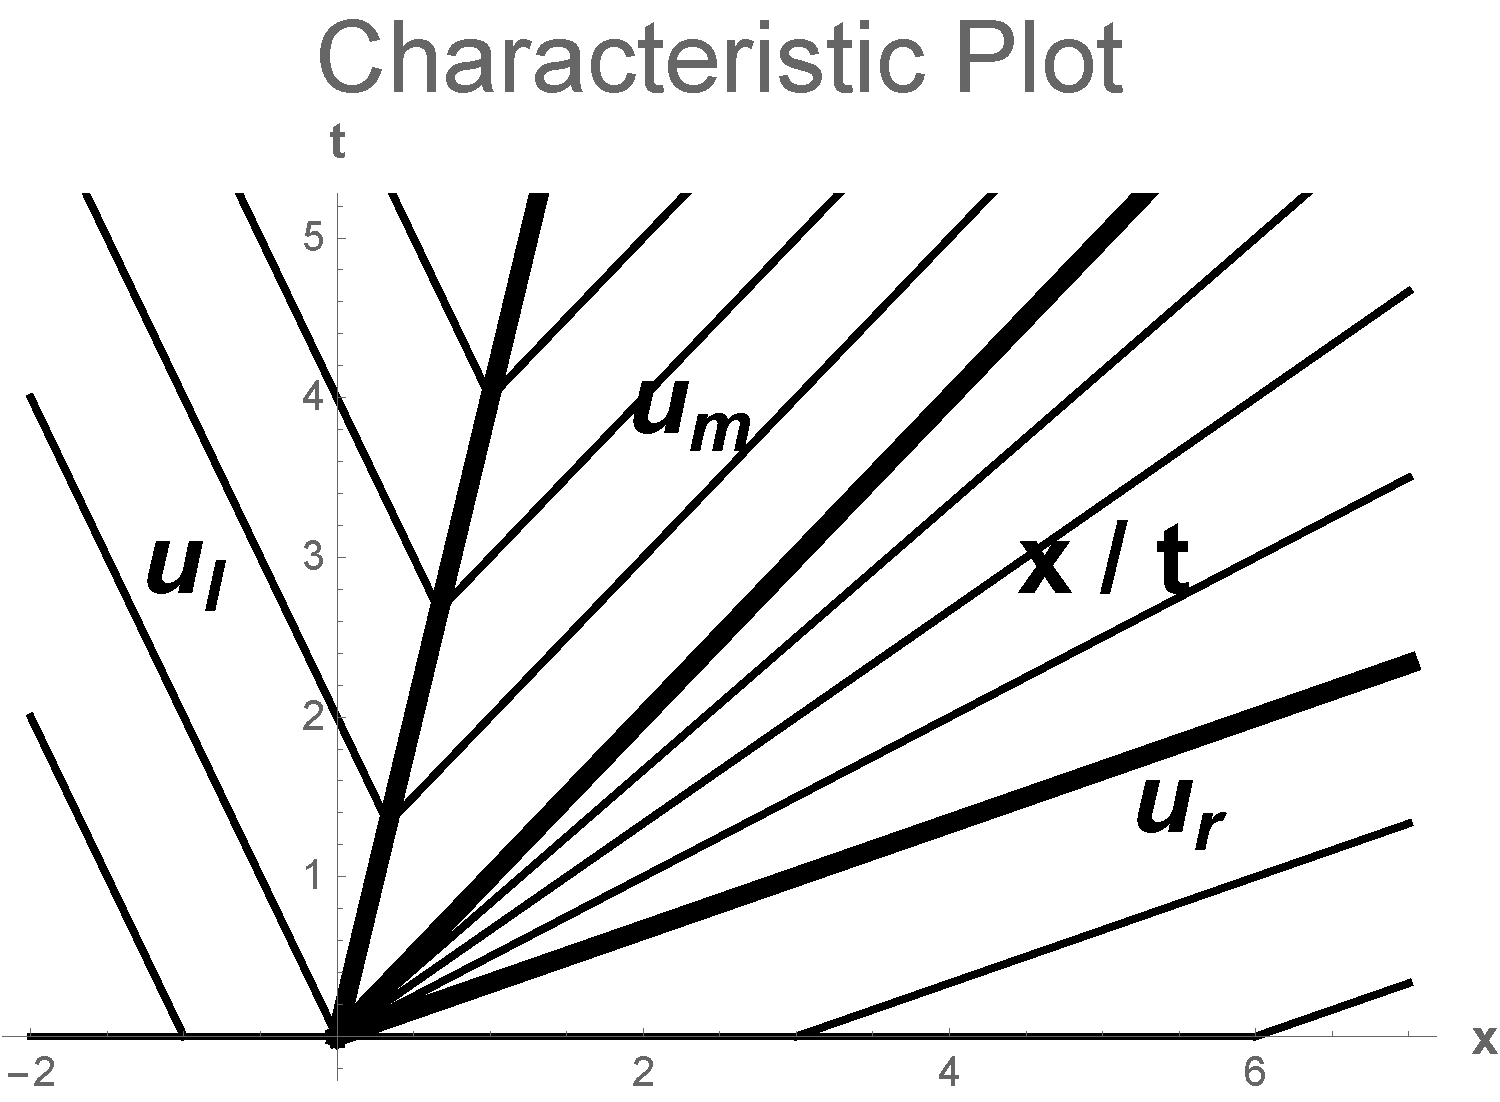
\includegraphics[scale=.6]{Figures/01_07.pdf}
    \end{center}

    %\begin{align*}
      %\dintt{0}{\infty}{\dintt{-\infty}{\infty}{u \phi_t}{x}}{t} &= \dintt{-\infty}{\infty}{\dintt{0}{\infty}{u \phi_t}{t}}{x} \\
      %&= \dintt{-\infty}{\infty}{\eval{u \phi}{t = 0}{\infty} - \dintt{0}{\infty}{u_t \phi}{t}}{x} \\
      %\intertext{Since $\phi$ has compact support, $\eval{\phi}{t = \infty}{} = 0$}
      %&= \dintt{-\infty}{\infty}{u(x, 0) \phi(x,0)}{x} - \dintt{-\infty}{\infty}{\dintt{0}{\infty}{u_t \phi}{t}}{x} \\
    %\end{align*}
    %Now I will just consider
    %\[
      %\dintt{-\infty}{\infty}{\dintt{0}{\infty}{u_t \phi}{t}}{x}
    %\]
    %I will only consider the case where $s_m > 0$, this implies that $0 < u_m < u_r$.
    %$u_l$ may be positive or negative but it is large enough that $s_m > 0$.
    %The other cases are roughly equivalent and would be redundant to fully write up.
    %In this case we can revisit the previous integral split it up into left and
    %right quadrants as follows.
    %\begin{align*}
      %\dintt{-\infty}{\infty}{\dintt{0}{\infty}{u_t \phi}{t}}{x} &= \dintt{-\infty}{0}{\dintt{0}{\infty}{\pda{u_l}{t} \phi}{t}}{x} + \dintt{0}{\infty}{\dintt{0}{\infty}{u_t \phi}{t}}{x} \\
      %&= \dintt{-\infty}{0}{\dintt{0}{\infty}{0 \times \phi}{t}}{x} + \dintt{0}{\infty}{\dintt{0}{\infty}{u_t \phi}{t}}{x} \\
      %&= \dintt{0}{\infty}{\dintt{0}{\infty}{u_t \phi}{t}}{x}
    %\end{align*}
    %Now the right quadrant can be split up into four sections based on time
    %\begin{align*}
      %&= \dintt*{0}{\infty}{\dintt{0}{x/u_r}{\pda{u_r}{t} \phi}{t} + \dintt{x/u_r}{x/u_m}{\pda{\frac{x}{t}}{t} \phi}{t} + \dintt{x/u_m}{x/s_m}{\pda{u_m}{t} \phi}{t} + \dintt{x/s_m}{\infty}{\pda{u_l}{t} \phi}{t}}{x} \\
      %&= \dintt*{0}{\infty}{\dintt{0}{x/u_r}{0 \times \phi}{t} + \dintt{x/u_r}{x/u_m}{-\frac{x}{t^2} \phi}{t} + \dintt{x/u_m}{x/s_m}{0 \times \phi}{t} + \dintt{x/s_m}{\infty}{0 \times \phi}{t}}{x} \\
      %&= \dintt{0}{\infty}{\dintt{x/u_r}{x/u_m}{-\frac{x}{t^2} \phi}{t}}{x}
    %\end{align*}

    %Next I will consider the term with the partial derivative in $x$.
    %\[
      %\dintt{0}{\infty}{\dintt{-\infty}{\infty}{\frac{1}{2}u^2 \phi_x}{x}}{t}
    %\]
    %Again this can be simplified by integrating by parts and substituting in for $u$.
    %\begin{gather*}
      %\dintt{0}{\infty}{\dintt{-\infty}{\infty}{\frac{1}{2}u^2 \phi_x}{x}}{t} = \dintt{0}{\infty}{\eval{\frac{1}{2}u^2 \phi}{x = -\infty}{\infty} - \dintt{-\infty}{\infty}{u u_x \phi}{x}}{t}
    %\end{gather*}
    %Since $\phi$ has compact support $\phi(\infty, t) = \phi(-\infty, t) = 0$
    %\begin{align*}
      %&= \dintt{0}{\infty}{0 - \dintt{-\infty}{\infty}{u u_x \phi}{x}}{t} \\
      %&= -\dintt*{0}{\infty}{\dintt{-\infty}{s_m t}{u_l \pda{u_l}{x} \phi}{x} + \dintt{s_m t}{u_m t}{u_m \pda{u_m}{x} \phi}{x} + \dintt{u_m t}{u_r t}{\frac{x}{t} \pda{\frac{x}{t}}{x} \phi}{x} + \dintt{u_r t }{\infty}{u_r \pda{u_r}{x} \phi}{x}}{t} \\
      %&= -\dintt*{0}{\infty}{\dintt{-\infty}{s_m t}{u_l \times 0 \times \phi}{x} + \dintt{s_m t}{u_m t}{u_m \times 0 \times \phi}{x} + \dintt{u_m t}{u_r t}{\frac{x}{t} \frac{1}{t} \phi}{x} + \dintt{u_r t }{\infty}{u_r \times 0 \times  \phi}{x}}{t} \\
      %&= -\dintt{0}{\infty}{\dintt{u_m t}{u_r t}{\frac{x}{t^2} \phi}{x}}{t}
    %\end{align*}


  \item % #4 Done
    I implemented a Forward Euler Upwind method in the following \MATLAB{} function.
    \lstinputlisting[language=MATLAB]{upwind.m}
    The following script uses the previous function to simulate a square wave
    propagating with periodic boundary conditions.
    \lstinputlisting[language=MATLAB]{H01.m}
    The following image is produced.
    Note that as time increases the solution decays more and more from the exact solution
    which is a perfect square wave.
    \begin{center}
      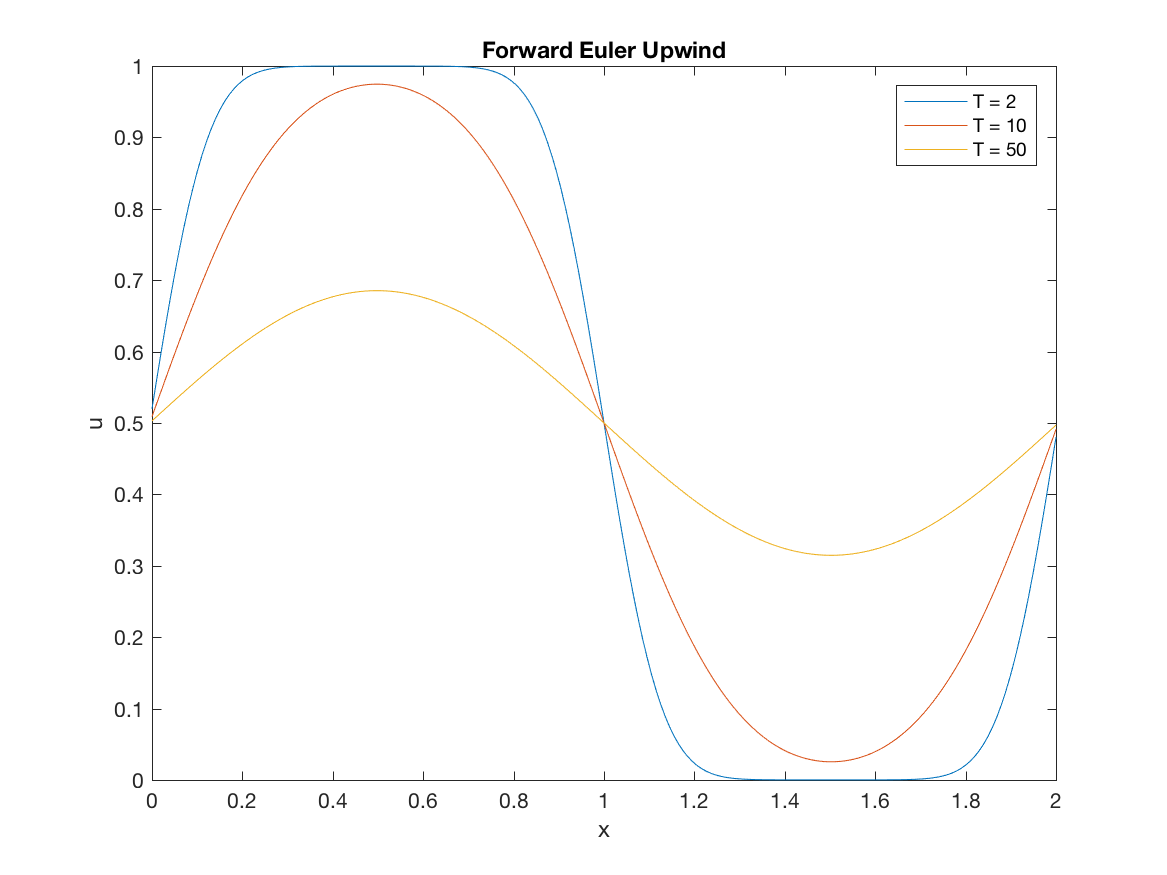
\includegraphics[scale=.8]{Figures/01_02.png}
    \end{center}


\end{enumerate}
\end{document}
